\documentclass{beamer}
\usepackage[utf8]{inputenc}
\usepackage{listings}
\usepackage{xcolor}
\usepackage{hyperref}
\usepackage{tikz}
\usetikzlibrary{shapes.geometric, arrows.meta, positioning}

\usetheme{Madrid}
\hypersetup{breaklinks=true}

% Python code style
\definecolor{codegray}{rgb}{0.95,0.95,0.95}
\definecolor{keyword}{rgb}{0.0,0.0,0.6}
\definecolor{comment}{rgb}{0.0,0.5,0.0}
\definecolor{string}{rgb}{0.64,0.08,0.08}

\lstdefinestyle{codeStyle}{
    language=Python,
    backgroundcolor=\color{codegray},
    commentstyle=\color{comment}\itshape,
    keywordstyle=\color{keyword}\bfseries,
    stringstyle=\color{string},
    basicstyle=\ttfamily\footnotesize,
    breaklines=true,
    frame=single,
    showstringspaces=false,
    tabsize=4,
    morekeywords={self, True, False, None, with, as, match, case}
}

% TikZ styles for flowcharts
\tikzset{
    startstop/.style={rectangle, rounded corners, draw, fill=blue!20, minimum width=2cm, minimum height=0.6cm},
    decision/.style={diamond, draw, fill=yellow!20, aspect=2, minimum width=1.5cm},
    process/.style={rectangle, draw, fill=green!10, minimum width=2cm, minimum height=0.6cm},
    arrow/.style={-{Stealth}, thick}
}

\title{Python for Cheminformatics \& Bioinformatics}
\subtitle{Lessons: Theory \& Concepts}
\author{Nirajan Bhattarai}
\institute{AI-Driven Drug Development Training}
\date{February 2026}

\begin{document}

% ============================================
% Title Slide
% ============================================
\begin{frame}
    \titlepage
\end{frame}

% ============================================
% Lessons Overview
% ============================================
\begin{frame}{Lessons Overview}
    \tableofcontents
\end{frame}

% ============================================
% Learning Objectives
% ============================================
\begin{frame}{Learning Objectives}
    \textbf{By the end of this course, you will be able to:}
    \vspace{0.5em}
    \begin{enumerate}
        \item Write Python code for basic data manipulation
        \item Work with molecular data (SMILES, formulas, properties)
        \item Process biological sequences (DNA, RNA, protein)
        \item Use control flow (conditionals, loops) for data filtering
        \item Organize data using lists, dictionaries, and sets
        \item Create reusable functions for cheminformatics tasks
        \item Read/write files (CSV, FASTA, JSON)
        \item Use NumPy arrays and Pandas DataFrames
        \item Apply concepts to Rosalind bioinformatics problems
    \end{enumerate}
\end{frame}

% ============================================
% Prerequisites
% ============================================
\begin{frame}{Prerequisites \& Setup}
    \textbf{Prerequisites:}
    \begin{itemize}
        \item Basic computer literacy
        \item No prior programming experience required
        \item Interest in drug discovery / life sciences
    \end{itemize}
    \vspace{1em}
    \textbf{Software Setup:}
    \begin{itemize}
        \item Python 3.8+ installed
        \item IDE: VS Code, PyCharm, or Jupyter Notebook
        \item Libraries: \texttt{pip install numpy pandas}
    \end{itemize}
    \vspace{1em}
    \textbf{Resources:}
    \begin{itemize}
        \item Rosalind.info -- Bioinformatics problems
        \item ChEMBL -- Bioactivity database
        \item PubChem -- Chemical information
    \end{itemize}
\end{frame}

% ============================================
% PREREQUISITE: DATA TYPES IN DRUG DISCOVERY
% ============================================
\section{Data Types in Drug Discovery}

% --------------------------------------------
% OVERVIEW SLIDE
% --------------------------------------------
\begin{frame}{Data Types You'll Encounter}
    \small
    \textbf{Before we start coding, let's understand the data types used in drug discovery:}
    \vspace{0.5em}
    \begin{columns}[T]
        \begin{column}{0.48\textwidth}
            \textbf{Cheminformatics:}
            \begin{itemize}
                \item SMILES -- Molecular structures
                \item Molecular Descriptors (MW, LogP)
                \item Activity Data (IC50, pIC50)
                \item Lipinski Properties
            \end{itemize}
        \end{column}
        \begin{column}{0.48\textwidth}
            \textbf{Bioinformatics:}
            \begin{itemize}
                \item DNA Sequences (A, T, G, C)
                \item RNA Sequences (A, U, G, C)
                \item Protein Sequences (amino acids)
                \item FASTA Format
            \end{itemize}
        \end{column}
    \end{columns}
    \vspace{0.5em}
    \textit{Understanding these data types is essential for the exercises in this course.}
\end{frame}

% --------------------------------------------
% SMILES NOTATION
% --------------------------------------------
\begin{frame}{SMILES: Simplified Molecular Input Line Entry System}
    \small
    \textbf{What is SMILES?}\\
    A text-based notation for representing chemical structures as strings.
    \vspace{0.5em}
    
    \textbf{Key Rules:}
    \begin{itemize}
        \item Atoms: C, N, O, S, P, F, Cl, Br, I (organic subset)
        \item Bonds: single (default), double (=), triple (\#), aromatic (:)
        \item Rings: Numbers indicate ring closures (e.g., \texttt{c1ccccc1} = benzene)
        \item Branches: Parentheses for side chains (e.g., \texttt{CC(C)C} = isobutane)
        \item Aromatic: Lowercase letters (c, n, o, s)
    \end{itemize}
    \vspace{0.5em}
    
    \textbf{Examples:}
    \begin{tabular}{ll}
        \texttt{CCO} & Ethanol \\
        \texttt{CC(=O)O} & Acetic acid \\
        \texttt{c1ccccc1} & Benzene \\
        \texttt{CC(=O)Oc1ccccc1C(=O)O} & Aspirin \\
    \end{tabular}
\end{frame}

\begin{frame}{SMILES: Visual Examples}
    \small
    \begin{center}
        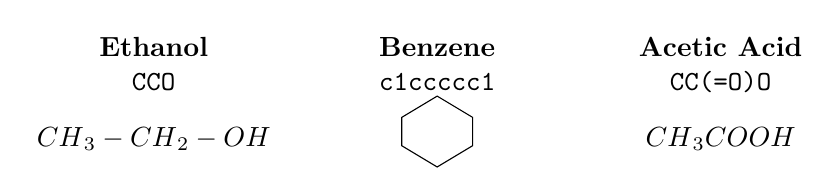
\begin{tikzpicture}[scale=0.9]
            % Ethanol
            \node at (0, 2.5) {\textbf{Ethanol}};
            \node at (0, 2) {\texttt{CCO}};
            \node at (0, 1.2) {$\text{CH}_3-\text{CH}_2-\text{OH}$};
            
            % Benzene
            \node at (4, 2.5) {\textbf{Benzene}};
            \node at (4, 2) {\texttt{c1ccccc1}};
            \draw (4, 0.8) -- (4.5, 1.1) -- (4.5, 1.5) -- (4, 1.8) -- (3.5, 1.5) -- (3.5, 1.1) -- cycle;
            
            % Acetic Acid
            \node at (8, 2.5) {\textbf{Acetic Acid}};
            \node at (8, 2) {\texttt{CC(=O)O}};
            \node at (8, 1.2) {$\text{CH}_3\text{COOH}$};
        \end{tikzpicture}
    \end{center}
    \vspace{0.5em}
    
    \textbf{Why SMILES?}
    \begin{itemize}
        \item Compact text representation (easy to store in databases)
        \item Human and machine readable
        \item Standard input for cheminformatics tools (RDKit, OpenBabel)
        \item Enables molecular property calculations
    \end{itemize}
\end{frame}

% --------------------------------------------
% SMARTS NOTATION
% --------------------------------------------
\begin{frame}{SMARTS: SMILES Arbitrary Target Specification}
    \small
    \textbf{What is SMARTS?}\\
    A pattern matching language for substructure searching in molecules.
    \vspace{0.5em}
    
    \textbf{Key Features:}
    \begin{itemize}
        \item Extension of SMILES with wildcards and logic
        \item Used to define functional groups and pharmacophores
        \item Essential for filtering compound libraries
    \end{itemize}
    \vspace{0.3em}
    
    \textbf{SMARTS Operators:}
    \begin{tabular}{ll}
        \texttt{*} & Any atom \\
        \texttt{[!C]} & Not carbon \\
        \texttt{[\#7]} & Nitrogen (by atomic number) \\
        \texttt{[C,N]} & Carbon OR nitrogen \\
        \texttt{[C;R]} & Carbon in a ring \\
        \texttt{[\$(C=O)]} & Recursive SMARTS \\
    \end{tabular}
\end{frame}

\begin{frame}[fragile]{SMARTS: Common Patterns}
    \small
    \textbf{Functional Group SMARTS:}
    \vspace{0.3em}
    
    \begin{tabular}{lll}
        \textbf{Pattern} & \textbf{SMARTS} & \textbf{Description} \\
        \hline
        Hydroxyl & \texttt{[OX2H]} & Alcohol OH \\
        Carboxylic acid & \texttt{[CX3](=O)[OX2H1]} & COOH \\
        Primary amine & \texttt{[NX3;H2]} & NH$_2$ \\
        Carbonyl & \texttt{[CX3]=[OX1]} & C=O \\
        Aromatic ring & \texttt{[a]} & Any aromatic atom \\
        Halogen & \texttt{[F,Cl,Br,I]} & Any halogen \\
    \end{tabular}
    \vspace{0.5em}
    
    \textbf{Python Example (RDKit):}
    \begin{lstlisting}[style=codeStyle, basicstyle=\ttfamily\scriptsize]
from rdkit import Chem
mol = Chem.MolFromSmiles("CC(=O)O")  # Acetic acid
pattern = Chem.MolFromSmarts("[CX3](=O)[OX2H1]")
has_cooh = mol.HasSubstructMatch(pattern)  # True
    \end{lstlisting}
\end{frame}

% --------------------------------------------
% SELFIES NOTATION
% --------------------------------------------
\begin{frame}{SELFIES: Self-Referencing Embedded Strings}
    \small
    \textbf{What is SELFIES?}\\
    A 100\% robust molecular string representation for machine learning.
    \vspace{0.5em}
    
    \textbf{Key Advantages over SMILES:}
    \begin{itemize}
        \item \textbf{Always valid}: Every SELFIES string is a valid molecule
        \item \textbf{No syntax errors}: Perfect for generative models
        \item \textbf{Bijective}: One-to-one mapping to molecules
        \item \textbf{ML-friendly}: Ideal for VAEs, GANs, transformers
    \end{itemize}
    \vspace{0.3em}
    
    \textbf{Example Comparison:}
    \begin{tabular}{ll}
        \textbf{SMILES} & \textbf{SELFIES} \\
        \hline
        \texttt{CCO} & \texttt{[C][C][O]} \\
        \texttt{c1ccccc1} & \texttt{[C][=C][C][=C][C][=C][Ring1][=Branch1]} \\
        \texttt{CC(=O)O} & \texttt{[C][C][=Branch1][C][=O][O]} \\
    \end{tabular}
\end{frame}

\begin{frame}[fragile]{SELFIES: Python Usage}
    \small
    \textbf{Why SELFIES for Machine Learning?}
    \begin{itemize}
        \item Random mutations always produce valid molecules
        \item No need to validate generated strings
        \item Better for evolutionary algorithms and generative AI
    \end{itemize}
    \vspace{0.3em}
    
    \textbf{Python Example:}
    \begin{lstlisting}[style=codeStyle, basicstyle=\ttfamily\scriptsize]
import selfies as sf

# SMILES to SELFIES
smiles = "CC(=O)Oc1ccccc1C(=O)O"  # Aspirin
selfies = sf.encoder(smiles)
print(selfies)
# [C][C][=Branch1][C][=O][O][C][=C][C][=C]...

# SELFIES to SMILES
recovered = sf.decoder(selfies)
print(recovered)  # CC(=O)Oc1ccccc1C(=O)O

# Get alphabet for tokenization
alphabet = sf.get_alphabet_from_selfies([selfies])
    \end{lstlisting}
    
    \vspace{0.2em}
    \textit{Install: \texttt{pip install selfies}}
\end{frame}

% --------------------------------------------
% InChI NOTATION
% --------------------------------------------
\begin{frame}{InChI: International Chemical Identifier}
    \small
    \textbf{What is InChI?}\\
    A standardized, unique identifier for chemical substances by IUPAC.
    \vspace{0.5em}
    
    \textbf{Structure:} \texttt{InChI=1S/formula/connections/h/...}
    \vspace{0.3em}
    
    \textbf{Layers:}
    \begin{itemize}
        \item \textbf{Formula}: Molecular formula (e.g., C9H8O4)
        \item \textbf{Connections}: Atom connectivity
        \item \textbf{H-atoms}: Hydrogen atom positions
        \item \textbf{Charge/Stereo}: Optional stereochemistry
    \end{itemize}
    \vspace{0.3em}
    
    \textbf{Example (Aspirin):}\\
    \texttt{\footnotesize InChI=1S/C9H8O4/c1-6(10)13-8-5-3-2-4-7(8)9(11)12/h2-5H,1H3,(H,11,12)}
    \vspace{0.3em}
    
    \textbf{InChIKey}: 27-character hash for database lookup\\
    \texttt{BSYNRYMUTXBXSQ-UHFFFAOYSA-N}
\end{frame}

\begin{frame}{InChI vs SMILES: When to Use Which?}
    \small
    \begin{tabular}{lll}
        \textbf{Feature} & \textbf{SMILES} & \textbf{InChI} \\
        \hline
        Uniqueness & Not canonical* & Canonical \\
        Human readable & Yes & Partially \\
        Database key & No & Yes (InChIKey) \\
        Substructure search & Yes & No \\
        Round-trip conversion & Yes & Lossy \\
        ML/AI input & Common & Rare \\
        Web search & Difficult & Easy (InChIKey) \\
    \end{tabular}
    \vspace{0.5em}
    
    \textit{*Canonical SMILES exist but vary by toolkit}
    \vspace{0.3em}
    
    \textbf{Best Practices:}
    \begin{itemize}
        \item Use \textbf{SMILES} for cheminformatics workflows
        \item Use \textbf{InChIKey} for database lookups and deduplication
        \item Use \textbf{SELFIES} for generative machine learning
        \item Use \textbf{SMARTS} for substructure filtering
    \end{itemize}
\end{frame}

% --------------------------------------------
% OTHER REPRESENTATIONS
% --------------------------------------------
\begin{frame}{Other Molecular Representations}
    \small
    \textbf{Molecular Fingerprints (for similarity):}
    \begin{itemize}
        \item \textbf{ECFP/Morgan}: Circular fingerprints (most common)
        \item \textbf{MACCS}: 166 predefined structural keys
        \item \textbf{RDKit FP}: Topological fingerprints
        \item \textbf{Atom-pair}: Pairs of atoms with distance
    \end{itemize}
    \vspace{0.3em}
    
    \textbf{3D Representations:}
    \begin{itemize}
        \item \textbf{SDF/MOL}: 3D coordinates + connectivity
        \item \textbf{PDB}: Protein Data Bank format
        \item \textbf{XYZ}: Simple coordinate format
    \end{itemize}
    \vspace{0.3em}
    
    \textbf{Graph Representations (for GNNs):}
    \begin{itemize}
        \item \textbf{Adjacency matrix}: Atom connectivity
        \item \textbf{Node features}: Atom types, charges
        \item \textbf{Edge features}: Bond types, orders
    \end{itemize}
\end{frame}

\begin{frame}{Molecular Representations: Summary}
    \small
    \begin{center}
        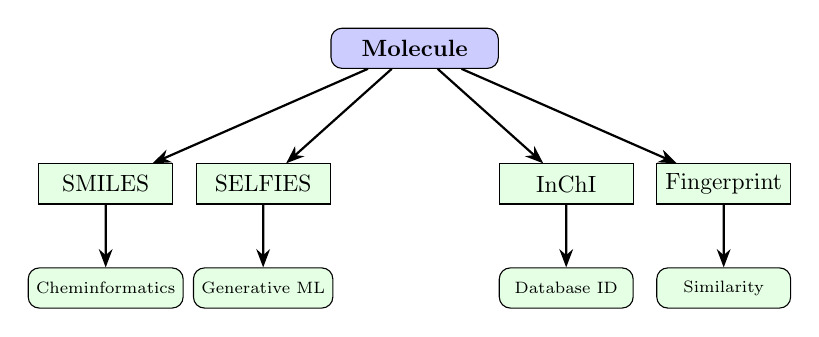
\begin{tikzpicture}[node distance=1.5cm, scale=0.85, every node/.style={scale=0.85}]
            \node (mol) [startstop, fill=blue!20, minimum width=2.5cm] {\textbf{Molecule}};
            
            \node (smiles) [process, below left=1.2cm and 2cm of mol] {SMILES};
            \node (selfies) [process, below left=1.2cm and 0cm of mol] {SELFIES};
            \node (inchi) [process, below right=1.2cm and 0cm of mol] {InChI};
            \node (fp) [process, below right=1.2cm and 2cm of mol] {Fingerprint};
            
            \node (use1) [startstop, fill=green!10, below=0.8cm of smiles, minimum width=2cm, font=\scriptsize] {Cheminformatics};
            \node (use2) [startstop, fill=green!10, below=0.8cm of selfies, minimum width=2cm, font=\scriptsize] {Generative ML};
            \node (use3) [startstop, fill=green!10, below=0.8cm of inchi, minimum width=2cm, font=\scriptsize] {Database ID};
            \node (use4) [startstop, fill=green!10, below=0.8cm of fp, minimum width=2cm, font=\scriptsize] {Similarity};
            
            \draw[arrow] (mol) -- (smiles);
            \draw[arrow] (mol) -- (selfies);
            \draw[arrow] (mol) -- (inchi);
            \draw[arrow] (mol) -- (fp);
            
            \draw[arrow] (smiles) -- (use1);
            \draw[arrow] (selfies) -- (use2);
            \draw[arrow] (inchi) -- (use3);
            \draw[arrow] (fp) -- (use4);
        \end{tikzpicture}
    \end{center}
    \vspace{0.3em}
    
    \textbf{Quick Reference:}
    \begin{tabular}{ll}
        \textbf{Task} & \textbf{Use} \\
        Property calculation & SMILES + RDKit \\
        Molecule generation & SELFIES \\
        Database search & InChIKey \\
        Similarity search & Morgan/ECFP fingerprints \\
        Pattern matching & SMARTS \\
    \end{tabular}
\end{frame}

% --------------------------------------------
% MOLECULAR DESCRIPTORS
% --------------------------------------------
\begin{frame}{Molecular Descriptors \& Properties}
    \small
    \textbf{Key Molecular Properties:}
    \vspace{0.3em}
    
    \begin{tabular}{lll}
        \textbf{Property} & \textbf{Description} & \textbf{Typical Range} \\
        \hline
        MW & Molecular Weight (Da) & 150--500 Da \\
        LogP & Lipophilicity (octanol/water) & -2 to 5 \\
        HBD & H-bond Donors & 0--5 \\
        HBA & H-bond Acceptors & 0--10 \\
        TPSA & Topological Polar Surface Area & 0--140 \AA$^2$ \\
        RotBonds & Rotatable Bonds & 0--10 \\
    \end{tabular}
    \vspace{0.5em}
    
    \textbf{Lipinski's Rule of Five (Drug-likeness):}
    \begin{itemize}
        \item MW $\leq$ 500 Da
        \item LogP $\leq$ 5
        \item HBD $\leq$ 5
        \item HBA $\leq$ 10
    \end{itemize}
    \textit{Compounds with $\leq$1 violation are likely orally bioavailable.}
\end{frame}

% --------------------------------------------
% ACTIVITY DATA
% --------------------------------------------
\begin{frame}{Bioactivity Data: IC50, Ki, and pIC50}
    \small
    \textbf{Measuring Drug Potency:}
    \vspace{0.3em}
    
    \begin{itemize}
        \item \textbf{IC50}: Concentration for 50\% inhibition
        \item \textbf{Ki}: Inhibition constant (binding affinity)
        \item \textbf{EC50}: Concentration for 50\% effect (agonists)
    \end{itemize}
    \vspace{0.3em}
    
    \textbf{Units:} Usually reported in nM (nanomolar) or $\mu$M (micromolar)
    \vspace{0.5em}
    
    \textbf{pIC50 Conversion:}
    \begin{equation*}
        \text{pIC50} = -\log_{10}(\text{IC50}_{\text{M}}) = 9 - \log_{10}(\text{IC50}_{\text{nM}})
    \end{equation*}
    \vspace{0.3em}
    
    \textbf{Activity Classification:}
    \begin{tabular}{lll}
        \textbf{pIC50} & \textbf{IC50 (nM)} & \textbf{Classification} \\
        \hline
        $\geq$ 8 & $\leq$ 10 & Highly Active \\
        6--8 & 10--1000 & Active \\
        5--6 & 1000--10000 & Moderate \\
        $<$ 5 & $>$ 10000 & Inactive \\
    \end{tabular}
\end{frame}

% --------------------------------------------
% DNA SEQUENCES
% --------------------------------------------
\begin{frame}{DNA: Deoxyribonucleic Acid}
    \small
    \textbf{The Blueprint of Life:}
    \begin{itemize}
        \item Double helix structure
        \item Four nucleotides: \textbf{A}denine, \textbf{T}hymine, \textbf{G}uanine, \textbf{C}ytosine
        \item Base pairing: A--T (2 H-bonds), G--C (3 H-bonds)
        \item Direction: 5' $\to$ 3' (reading direction)
    \end{itemize}
    \vspace{0.3em}
    
    \begin{center}
        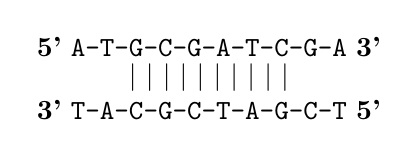
\begin{tikzpicture}[scale=0.8]
            \node at (0, 1.5) {\textbf{5'} \texttt{A-T-G-C-G-A-T-C-G-A} \textbf{3'}};
            \node at (0, 1.0) {$|$ $|$ $|$ $|$ $|$ $|$ $|$ $|$ $|$ $|$};
            \node at (0, 0.5) {\textbf{3'} \texttt{T-A-C-G-C-T-A-G-C-T} \textbf{5'}};
        \end{tikzpicture}
    \end{center}
    \vspace{0.3em}
    
    \textbf{Key Metrics:}
    \begin{itemize}
        \item \textbf{GC Content}: \% of G and C bases (stability indicator)
        \item \textbf{Length}: Number of base pairs (bp) or nucleotides (nt)
        \item \textbf{Codons}: 3-nucleotide sequences encoding amino acids
    \end{itemize}
\end{frame}

% --------------------------------------------
% RNA SEQUENCES
% --------------------------------------------
\begin{frame}{RNA: Ribonucleic Acid}
    \small
    \textbf{DNA's Working Copy:}
    \begin{itemize}
        \item Single-stranded molecule
        \item Four nucleotides: \textbf{A}denine, \textbf{U}racil, \textbf{G}uanine, \textbf{C}ytosine
        \item \textbf{Key difference}: Uracil (U) replaces Thymine (T)
    \end{itemize}
    \vspace{0.3em}
    
    \textbf{Transcription (DNA $\to$ RNA):}
    \begin{center}
        \texttt{DNA: ATGCGATCG} $\rightarrow$ \texttt{RNA: AUGCGAUCG}
    \end{center}
    \vspace{0.3em}
    
    \textbf{Types of RNA:}
    \begin{tabular}{ll}
        \textbf{mRNA} & Messenger RNA (carries genetic code) \\
        \textbf{tRNA} & Transfer RNA (brings amino acids) \\
        \textbf{rRNA} & Ribosomal RNA (protein synthesis) \\
        \textbf{siRNA} & Small interfering RNA (gene silencing) \\
    \end{tabular}
    \vspace{0.3em}
    
    \textit{In Python: \texttt{rna = dna.replace("T", "U")}}
\end{frame}

% --------------------------------------------
% PROTEIN SEQUENCES
% --------------------------------------------
\begin{frame}{Proteins: Amino Acid Sequences}
    \small
    \textbf{The Workhorses of the Cell:}
    \begin{itemize}
        \item Built from 20 standard amino acids
        \item Encoded by codons (3 nucleotides = 1 amino acid)
        \item \textbf{Start codon}: AUG (Methionine)
        \item \textbf{Stop codons}: UAA, UAG, UGA
    \end{itemize}
    \vspace{0.3em}
    
    \textbf{Translation (RNA $\to$ Protein):}
    \begin{center}
        \texttt{AUG-GCC-UAU-...-UAA} $\rightarrow$ \texttt{M-A-Y-...}
    \end{center}
    \vspace{0.3em}
    
    \textbf{Amino Acid Properties:}
    \begin{tabular}{ll}
        \textbf{Hydrophobic} & A, V, L, I, M, F, W, P \\
        \textbf{Polar} & S, T, N, Q, Y, C \\
        \textbf{Charged (+)} & K, R, H \\
        \textbf{Charged (-)} & D, E \\
        \textbf{Special} & G (flexible), P (rigid) \\
    \end{tabular}
\end{frame}

% --------------------------------------------
% FASTA FORMAT
% --------------------------------------------
\begin{frame}[fragile]{FASTA Format: Sequence Storage}
    \small
    \textbf{Standard Format for Biological Sequences:}
    \vspace{0.3em}
    
    \begin{lstlisting}[style=codeStyle, basicstyle=\ttfamily\scriptsize]
>Rosalind_6404 Human hemoglobin alpha
MVLSPADKTNVKAAWGKVGAHAGEYGAEALERMFLSFPTTKTYFPHFDLSH
GSAQVKGHGKKVADALTNAVAHVDDMPNALSALSDLHAHKLRVDPVNFKLL
SHCLLVTLAAHLPAEFTPAVHASLDKFLASVSTVLTSKYR
>Rosalind_5959 E. coli beta-galactosidase
MTMITDSLAVVLQRRDWENPGVTQLNRLAAHPPFASWRNSEEARTDRPSQQ
LRSLNGEWRFAWFPAPEAVPESWLECDLPEADTVVVPSNWQMHGYDAPIYT
    \end{lstlisting}
    \vspace{0.3em}
    
    \textbf{Format Rules:}
    \begin{itemize}
        \item Header line starts with \texttt{>} followed by sequence ID
        \item Sequence data on following lines (typically 60--80 chars/line)
        \item Multiple sequences in one file
    \end{itemize}
    \vspace{0.3em}
    
    \textit{Common source: \href{https://rosalind.info}{Rosalind.info} bioinformatics problems}
\end{frame}

% --------------------------------------------
% CENTRAL DOGMA SUMMARY
% --------------------------------------------
\begin{frame}{The Central Dogma of Molecular Biology}
    \small
    \begin{center}
        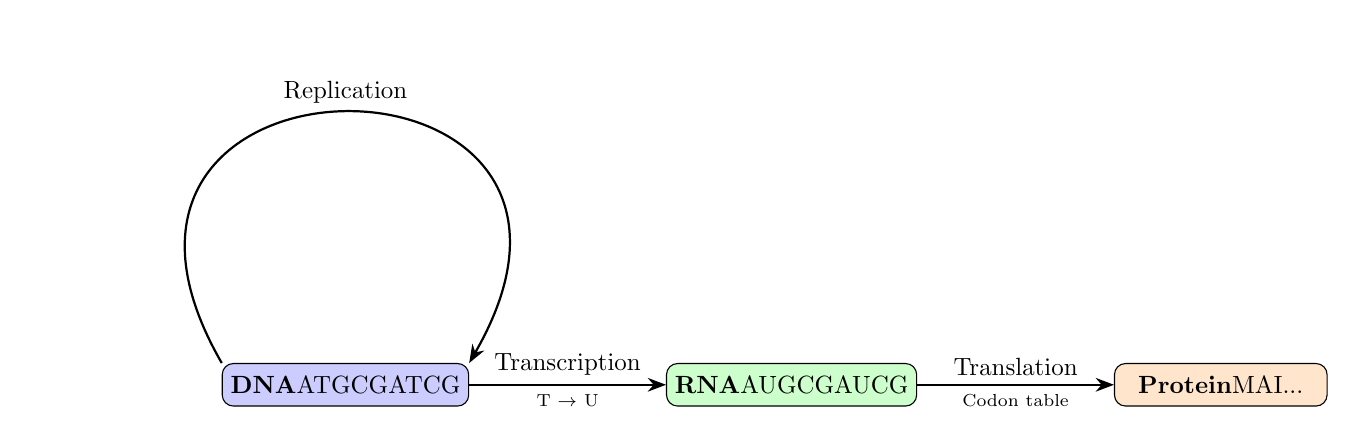
\begin{tikzpicture}[node distance=2.5cm, scale=0.9, every node/.style={scale=0.9}]
            \node (dna) [startstop, fill=blue!20, minimum width=3cm] {\textbf{DNA}\\ATGCGATCG};
            \node (rna) [startstop, fill=green!20, right=of dna, minimum width=3cm] {\textbf{RNA}\\AUGCGAUCG};
            \node (protein) [startstop, fill=orange!20, right=of rna, minimum width=3cm] {\textbf{Protein}\\MAI...};
            
            \draw[arrow] (dna) -- node[above] {Transcription} node[below] {\scriptsize T $\to$ U} (rna);
            \draw[arrow] (rna) -- node[above] {Translation} node[below] {\scriptsize Codon table} (protein);
            
            % Replication arrow (loop above DNA)
            \draw[arrow] (dna.north west) to[out=120,in=60,looseness=4] node[above] {Replication} (dna.north east);
        \end{tikzpicture}
    \end{center}
    \vspace{0.5em}
    
    \textbf{Key Operations in Bioinformatics:}
    \begin{itemize}
        \item \textbf{Transcribe}: DNA $\to$ RNA (replace T with U)
        \item \textbf{Translate}: RNA $\to$ Protein (use codon table)
        \item \textbf{Reverse Complement}: Get complementary DNA strand
        \item \textbf{GC Content}: Calculate sequence stability
    \end{itemize}
\end{frame}

% --------------------------------------------
% SUMMARY TABLE
% --------------------------------------------
\begin{frame}{Summary: Data Types Reference}
    \small
    \begin{tabular}{lll}
        \textbf{Data Type} & \textbf{Python Type} & \textbf{Example} \\
        \hline
        SMILES & \texttt{str} & \texttt{"CC(=O)Oc1ccccc1C(=O)O"} \\
        MW & \texttt{float} & \texttt{180.16} \\
        LogP & \texttt{float} & \texttt{1.19} \\
        IC50 (nM) & \texttt{float} & \texttt{5.2} \\
        pIC50 & \texttt{float} & \texttt{8.28} \\
        Drug-like & \texttt{bool} & \texttt{True} \\
        \hline
        DNA sequence & \texttt{str} & \texttt{"ATGCGATCG"} \\
        RNA sequence & \texttt{str} & \texttt{"AUGCGAUCG"} \\
        Protein sequence & \texttt{str} & \texttt{"MAMAPRTEIN"} \\
        GC content & \texttt{float} & \texttt{55.5} \\
        Sequence length & \texttt{int} & \texttt{1542} \\
    \end{tabular}
    \vspace{0.5em}
    
    \textit{All biological sequences are strings in Python!}
\end{frame}

% ============================================
% SECTION 1: BASICS
% ============================================
\section{Python Basics}

% --------------------------------------------
% LESSON 1: VARIABLES & DATA TYPES
% --------------------------------------------
\begin{frame}{Lesson 1: Learning Objectives}
    \small
    \textbf{Learning Objectives:}
    \begin{itemize}
        \item Understand how variables store data in memory
        \item Identify Python's core data types (int, float, str, bool)
        \item Perform type conversions between data types
    \end{itemize}
    \vspace{0.5em}
    \textbf{Description:}\\
    Variables are the foundation of programming -- named containers that hold data. Understanding data types ensures correct operations and prevents errors in scientific computing.
    \vspace{0.5em}
    \textbf{Applications:}
    \begin{itemize}
        \item Store compound properties (MW, LogP, SMILES)
        \item Represent bioactivity measurements (IC50, pIC50)
        \item Handle DNA/RNA sequence data
    \end{itemize}
\end{frame}

\begin{frame}{Lesson 1: Variables \& Data Types}
    \small
    \textbf{Concept:} Variables store data in memory.\\[0.5em]
    Python data types: \texttt{int}, \texttt{float}, \texttt{str}, \texttt{bool}, \texttt{NoneType}\\[0.5em]
    \textbf{Type Conversion:} \texttt{int()}, \texttt{float()}, \texttt{str()}, \texttt{bool()}\\[0.5em]
    \textbf{Drug Discovery Scenarios:}
    \begin{itemize}
        \item Compound Info (name, MW, LogP, SMILES)
        \item Bioactivity Data (IC50, Ki, pIC50)
        \item DNA/RNA Sequences (nucleotide strings)
    \end{itemize}
\end{frame}

\begin{frame}[fragile]{Lesson 1 Code Example}
    \small
    \begin{lstlisting}[style=codeStyle]
# Compound Info
compound_name = "Aspirin"
mw = 180.16  # Molecular Weight (Da)
logP = 1.19  # Lipophilicity
smiles = "CC(=O)OC1=CC=CC=C1C(=O)O"

# Bioactivity Data
ic50_nM = 5.2  # IC50 in nanomolar
pic50 = 8.28   # -log10(IC50 in M)
is_active = True

# DNA Sequence
dna_seq = "ATGCGATCGATCG"
seq_length = len(dna_seq)

# Type Conversion
ic50_str = str(ic50_nM)
mw_int = int(mw)

print(f"{compound_name}: MW={mw}, pIC50={pic50}")
    \end{lstlisting}
\end{frame}

% --------------------------------------------
% LESSON 2: OPERATORS
% --------------------------------------------
\begin{frame}{Lesson 2: Learning Objectives}
    \small
    \textbf{Learning Objectives:}
    \begin{itemize}
        \item Use arithmetic operators for scientific calculations
        \item Apply comparison operators to filter data
        \item Combine conditions using logical operators
    \end{itemize}
    \vspace{0.5em}
    \textbf{Description:}\\
    Operators are symbols that perform computations and comparisons. They enable mathematical transformations, data filtering, and decision-making in code.
    \vspace{0.5em}
    \textbf{Applications:}
    \begin{itemize}
        \item Convert IC50 to pIC50 ($-\log_{10}$)
        \item Check Lipinski Rule of Five compliance
        \item Calculate GC content in DNA sequences
    \end{itemize}
\end{frame}

\begin{frame}{Lesson 2: Operators}
    \small
    \textbf{Arithmetic:} \texttt{+}, \texttt{-}, \texttt{*}, \texttt{/}, \texttt{\%}, \texttt{**}\\[0.5em]
    \textbf{Comparison:} \texttt{>}, \texttt{<}, \texttt{==}, \texttt{!=}, \texttt{>=}, \texttt{<=}\\[0.5em]
    \textbf{Logical:} \texttt{and}, \texttt{or}, \texttt{not}\\[0.5em]
    \textbf{Drug Discovery scenarios:} Calculate pIC50, check Lipinski rules, filter active compounds
\end{frame}

\begin{frame}[fragile]{Lesson 2 Code Example}
    \small
    \begin{lstlisting}[style=codeStyle]
import math

# IC50 to pIC50 conversion
ic50_nM = 10.0  # nanomolar
ic50_M = ic50_nM * 1e-9  # convert to molar
pic50 = -math.log10(ic50_M)  # pIC50 = 8.0
print(f"IC50: {ic50_nM} nM -> pIC50: {pic50:.2f}")

# Lipinski Rule of Five checks
mw, logP, hbd, hba = 450, 3.5, 2, 6
lipinski_ok = (mw <= 500) and (logP <= 5) and (hbd <= 5) and (hba <= 10)
print(f"Passes Lipinski: {lipinski_ok}")

# GC Content calculation
seq = "ATGCGCGCTA"
gc_count = seq.count("G") + seq.count("C")
gc_percent = (gc_count / len(seq)) * 100
print(f"GC Content: {gc_percent:.1f}%")
    \end{lstlisting}
\end{frame}

% --------------------------------------------
% LESSON 3: STRINGS
% --------------------------------------------
\begin{frame}{Lesson 3: Learning Objectives}
    \small
    \textbf{Learning Objectives:}
    \begin{itemize}
        \item Manipulate strings using indexing and slicing
        \item Apply string methods for text processing
        \item Parse and transform sequence data
    \end{itemize}
    \vspace{0.5em}
    \textbf{Description:}\\
    Strings are sequences of characters essential for representing biological sequences (DNA, RNA, proteins) and chemical notations (SMILES). String manipulation is fundamental to bioinformatics.
    \vspace{0.5em}
    \textbf{Applications:}
    \begin{itemize}
        \item Transcribe DNA to RNA (T $\to$ U)
        \item Generate reverse complement sequences
        \item Parse SMILES for molecular features
    \end{itemize}
\end{frame}

\begin{frame}{Lesson 3: Strings}
    \small
    Strings store text -- essential for sequences and SMILES.\\[0.5em]
    \textbf{Methods:} indexing/slicing, \texttt{len()}, \texttt{upper()}, \texttt{lower()}, \texttt{replace()}, \texttt{split()}, \texttt{count()}, \texttt{find()}\\[0.5em]
    \textbf{Drug Discovery scenarios:} DNA/RNA sequences, SMILES strings, protein sequences
\end{frame}

\begin{frame}[fragile]{Lesson 3 Code Example}
    \small
    \begin{lstlisting}[style=codeStyle]
# DNA Sequence manipulation
dna = "ATGCGATCGATCG"
print(f"Length: {len(dna)}")
print(f"First 3 (codon): {dna[:3]}")  # ATG
print(f"Last codon: {dna[-3:]}")       # TCG

# Transcription: DNA -> RNA (T -> U)
rna = dna.replace("T", "U")
print(f"RNA: {rna}")  # AUGCGAUCGAUCG

# Count nucleotides
print(f"A: {dna.count('A')}, T: {dna.count('T')}")
print(f"G: {dna.count('G')}, C: {dna.count('C')}")

# SMILES analysis
smiles = "CC(=O)OC1=CC=CC=C1C(=O)O"
has_ring = any(c.isdigit() for c in smiles)
print(f"Has ring: {has_ring}")  # True
    \end{lstlisting}
\end{frame}

% --------------------------------------------
% LESSON 4: CONDITIONALS
% --------------------------------------------
\begin{frame}{Lesson 4: Learning Objectives}
    \small
    \textbf{Learning Objectives:}
    \begin{itemize}
        \item Control program flow with if/elif/else statements
        \item Use match-case for pattern matching (Python 3.10+)
        \item Build nested conditional logic
    \end{itemize}
    \vspace{0.5em}
    \textbf{Description:}\\
    Conditionals allow programs to make decisions based on data values. They enable classification, filtering, and rule-based logic essential for compound screening.
    \vspace{0.5em}
    \textbf{Applications:}
    \begin{itemize}
        \item Classify compounds by activity level
        \item Check drug-likeness (Lipinski violations)
        \item Identify start/stop codons in sequences
    \end{itemize}
\end{frame}

\begin{frame}{Lesson 4: Conditional Statements}
    \small
    \texttt{if}/\texttt{elif}/\texttt{else} for branching\\
    \texttt{match-case} (Python 3.10+) for pattern matching
    \vspace{0.5em}
    \begin{center}
        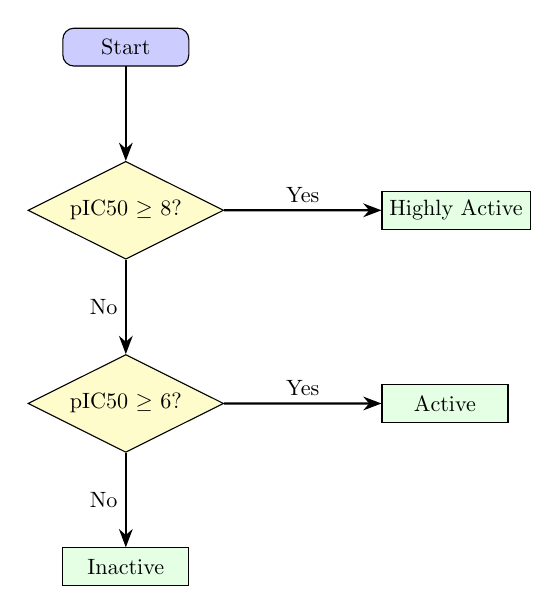
\begin{tikzpicture}[node distance=1.2cm, scale=0.8, every node/.style={scale=0.8}]
            \node (start) [startstop] {Start};
            \node (cond1) [decision, below=of start] {pIC50 $\geq$ 8?};
            \node (active) [process, right=2cm of cond1] {Highly Active};
            \node (cond2) [decision, below=of cond1] {pIC50 $\geq$ 6?};
            \node (moderate) [process, right=2cm of cond2] {Active};
            \node (inactive) [process, below=of cond2] {Inactive};
            
            \draw[arrow] (start) -- (cond1);
            \draw[arrow] (cond1) -- node[above] {Yes} (active);
            \draw[arrow] (cond1) -- node[left] {No} (cond2);
            \draw[arrow] (cond2) -- node[above] {Yes} (moderate);
            \draw[arrow] (cond2) -- node[left] {No} (inactive);
        \end{tikzpicture}
    \end{center}
\end{frame}

\begin{frame}[fragile]{Lesson 4 Code Example (if/else)}
    \small
    \begin{lstlisting}[style=codeStyle]
# Classify compound activity by pIC50
pic50 = 7.5
if pic50 >= 8:
    activity = "Highly Active"
elif pic50 >= 6:
    activity = "Active"
elif pic50 >= 5:
    activity = "Moderate"
else:
    activity = "Inactive"
print(f"pIC50 {pic50}: {activity}")

# Check Lipinski Rule of Five
mw, logP, hbd, hba = 450, 4.2, 2, 6
violations = 0
if mw > 500: violations += 1
if logP > 5: violations += 1
if hbd > 5: violations += 1
if hba > 10: violations += 1
drug_like = "Yes" if violations <= 1 else "No"
print(f"Drug-like: {drug_like} ({violations} violations)")
    \end{lstlisting}
\end{frame}

\begin{frame}[fragile]{Lesson 4 Code Example (match-case)}
    \small
    \begin{lstlisting}[style=codeStyle]
# Identify codon type (Python 3.10+)
codon = "ATG"
match codon:
    case "ATG":
        print("Start codon (Methionine)")
    case "TAA" | "TAG" | "TGA":
        print("Stop codon")
    case _:
        print("Coding codon")

# Classify nucleotide
nucleotide = "G"
match nucleotide:
    case "A" | "G":
        base_type = "Purine"
    case "C" | "T":
        base_type = "Pyrimidine"
    case _:
        base_type = "Unknown"
print(f"{nucleotide} is a {base_type}")
    \end{lstlisting}
\end{frame}

% --------------------------------------------
% LESSON 5: LOOPS
% --------------------------------------------
\begin{frame}{Lesson 5: Learning Objectives}
    \small
    \textbf{Learning Objectives:}
    \begin{itemize}
        \item Iterate over sequences using for loops
        \item Use while loops for conditional repetition
        \item Control loop flow with break and continue
    \end{itemize}
    \vspace{0.5em}
    \textbf{Description:}\\
    Loops automate repetitive tasks by executing code blocks multiple times. They are essential for processing compound libraries and analyzing sequence data at scale.
    \vspace{0.5em}
    \textbf{Applications:}
    \begin{itemize}
        \item Process compound libraries (batch MW calculation)
        \item Count nucleotide frequencies (Rosalind DNA)
        \item Screen compounds against activity thresholds
    \end{itemize}
\end{frame}

\begin{frame}{Lesson 5: Loops}
    \small
    \texttt{for} loop: iterate sequences/range\\
    \texttt{while} loop: repeat until condition False\\
    \texttt{break}/\texttt{continue}: control loop flow
    \vspace{0.5em}
    \begin{center}
        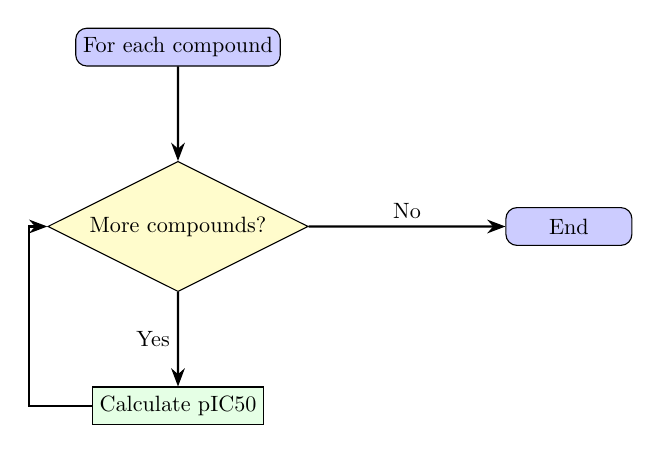
\begin{tikzpicture}[node distance=1.2cm, scale=0.8, every node/.style={scale=0.8}]
            \node (start) [startstop] {For each compound};
            \node (cond) [decision, below=of start] {More compounds?};
            \node (body) [process, below=of cond] {Calculate pIC50};
            \node (end) [startstop, right=2.5cm of cond] {End};
            
            \draw[arrow] (start) -- (cond);
            \draw[arrow] (cond) -- node[above] {No} (end);
            \draw[arrow] (cond) -- node[left] {Yes} (body);
            \draw[arrow] (body.west) -- ++(-1,0) |- (cond.west);
        \end{tikzpicture}
    \end{center}
\end{frame}

\begin{frame}[fragile]{Lesson 5 Code Example}
    \small
    \begin{lstlisting}[style=codeStyle]
import math

# Process compound library - calculate pIC50
ic50_values = [5.2, 120.0, 8.7, 2.1, 450.0]  # nM
for ic50 in ic50_values:
    pic50 = 9 - math.log10(ic50)
    print(f"IC50: {ic50:>6.1f} nM -> pIC50: {pic50:.2f}")

# Count nucleotides in DNA sequence
dna = "ATGCGATCGATCG"
counts = {"A": 0, "T": 0, "G": 0, "C": 0}
for nucleotide in dna:
    counts[nucleotide] += 1
print(f"Nucleotide counts: {counts}")

# Find active compounds (break/continue)
compounds = [("CPD1", 7.2), ("CPD2", 5.1), ("CPD3", 8.5)]
for name, pic50 in compounds:
    if pic50 < 6: continue  # skip inactive
    if pic50 > 8: break     # found highly active
    print(f"{name}: Active (pIC50={pic50})")
    \end{lstlisting}
\end{frame}

% --------------------------------------------
% LESSON 6: FUNCTIONS
% --------------------------------------------
\begin{frame}{Lesson 6: Learning Objectives}
    \small
    \textbf{Learning Objectives:}
    \begin{itemize}
        \item Define reusable functions with parameters
        \item Use return statements to output results
        \item Apply *args and **kwargs for flexible inputs
    \end{itemize}
    \vspace{0.5em}
    \textbf{Description:}\\
    Functions encapsulate reusable code blocks, promoting modularity and reducing duplication. They are the building blocks of scientific pipelines and analysis tools.
    \vspace{0.5em}
    \textbf{Applications:}
    \begin{itemize}
        \item Create IC50 $\to$ pIC50 converters
        \item Build Lipinski property calculators
        \item Implement sequence analysis functions (GC, REVC)
    \end{itemize}
\end{frame}

\begin{frame}{Lesson 6: Functions}
    \small
    \texttt{def name(params):} define function\\
    \texttt{return} for return value\\
    Default arguments, *args, **kwargs
    \vspace{0.5em}
    \begin{center}
        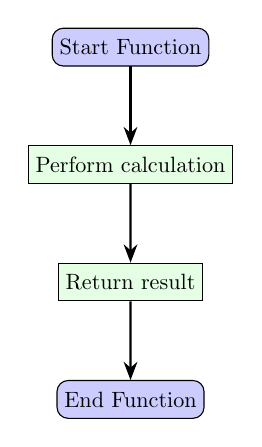
\begin{tikzpicture}[node distance=1cm, scale=0.8, every node/.style={scale=0.8}]
            \node (start) [startstop] {Start Function};
            \node (process) [process, below=of start] {Perform calculation};
            \node (return) [process, below=of process] {Return result};
            \node (end) [startstop, below=of return] {End Function};
            
            \draw[arrow] (start) -- (process);
            \draw[arrow] (process) -- (return);
            \draw[arrow] (return) -- (end);
        \end{tikzpicture}
    \end{center}
\end{frame}

\begin{frame}[fragile]{Lesson 6 Code Example}
    \small
    \begin{lstlisting}[style=codeStyle]
# Function: IC50 to pIC50 conversion
def ic50_to_pic50(ic50_nm):
    """Convert IC50 (nM) to pIC50."""
    return -math.log10(ic50_nm * 1e-9)

# Function with validation
def calculate_molecular_weight(smiles):
    """Calculate MW from SMILES."""
    mol = Chem.MolFromSmiles(smiles)
    if mol is None:
        return None, "Invalid SMILES"
    return Descriptors.MolWt(mol), "Success"

# *args - process multiple compounds
def average_activity(*pic50_values):
    return sum(pic50_values) / len(pic50_values)

# **kwargs - compound properties
def print_compound(**props):
    for key, value in props.items():
        print(f"{key}: {value}")

print(ic50_to_pic50(10))  # 8.0
    \end{lstlisting}
\end{frame}

% --------------------------------------------
% LESSON 6B: ERROR HANDLING
% --------------------------------------------
\begin{frame}{Lesson 6B: Learning Objectives}
    \small
    \textbf{Learning Objectives:}
    \begin{itemize}
        \item Handle runtime errors with try/except blocks
        \item Use else and finally for cleanup operations
        \item Raise custom exceptions for validation
    \end{itemize}
    \vspace{0.5em}
    \textbf{Description:}\\
    Error handling prevents program crashes from invalid data or unexpected conditions. Robust error handling is critical when processing real-world chemical/biological data with missing or malformed entries.
    \vspace{0.5em}
    \textbf{Applications:}
    \begin{itemize}
        \item Handle invalid SMILES parsing gracefully
        \item Manage missing data in compound datasets
        \item Validate FASTA file formats
    \end{itemize}
\end{frame}

\begin{frame}{Lesson 6B: Error Handling (try/except)}
    \small
    \textbf{Concept:} Handle runtime errors gracefully\\[0.5em]
    \textbf{Keywords:} \texttt{try}, \texttt{except}, \texttt{else}, \texttt{finally}, \texttt{raise}\\[0.5em]
    \textbf{Common Exceptions:}
    \begin{itemize}
        \item \texttt{ValueError} -- invalid value conversion
        \item \texttt{TypeError} -- wrong type operation
        \item \texttt{ZeroDivisionError} -- division by zero
        \item \texttt{FileNotFoundError} -- file doesn't exist
        \item \texttt{KeyError} -- dict key not found
        \item \texttt{IndexError} -- list index out of range
    \end{itemize}
\end{frame}

\begin{frame}[fragile]{Lesson 6B Code Example}
    \small
    \begin{lstlisting}[style=codeStyle]
# Basic try/except
try:
    num = int(input("Enter number: "))
    result = 10 / num
except ValueError:
    print("Invalid input!")
except ZeroDivisionError:
    print("Cannot divide by zero!")
else:
    print(f"Result: {result}")
finally:
    print("Execution complete")

# Raising exceptions
def divide(a, b):
    if b == 0:
        raise ValueError("Divisor cannot be zero")
    return a / b
    \end{lstlisting}
\end{frame}

% ============================================
% SECTION 2: COLLECTIONS AND ADVANCED CONCEPTS
% ============================================
\section{Collections and Advanced Python Concepts}

% --------------------------------------------
% LESSON 7: LISTS
% --------------------------------------------
\begin{frame}{Lesson 7: Learning Objectives}
    \small
    \textbf{Learning Objectives:}
    \begin{itemize}
        \item Create and modify lists using built-in methods
        \item Access elements via indexing and slicing
        \item Perform common list operations (append, remove, sort)
    \end{itemize}
    \vspace{0.5em}
    \textbf{Description:}\\
    Lists are ordered, mutable collections that store sequences of items. They are the primary data structure for managing compound libraries and activity datasets.
    \vspace{0.5em}
    \textbf{Applications:}
    \begin{itemize}
        \item Store SMILES strings for compound libraries
        \item Manage pIC50 activity measurements
        \item Build queues for batch processing
    \end{itemize}
\end{frame}

\begin{frame}{Lesson 7: Python Lists -- Basics}
    \small
    Lists store ordered sequences.\\[0.5em]
    \textbf{Methods:} \texttt{append}, \texttt{extend}, \texttt{insert}, \texttt{remove}, \texttt{pop}, \texttt{clear}, \texttt{index}, \texttt{count}, \texttt{copy}\\[0.5em]
    \textbf{Scenario Examples:} SMILES list, pIC50 values, compound IDs, sequence fragments
\end{frame}

\begin{frame}[fragile]{Lesson 7 Code Example}
    \small
    \begin{lstlisting}[style=codeStyle]
smiles_list = ["CCO", "CC(=O)O", "c1ccccc1"]
smiles_list.append("CCN")
smiles_list.insert(1, "CC")
smiles_list.remove("CCO")
print(smiles_list[0], smiles_list[-1])
    \end{lstlisting}
\end{frame}

% --------------------------------------------
% LESSON 7B: TUPLES & SETS
% --------------------------------------------
\begin{frame}{Lesson 7B: Learning Objectives}
    \small
    \textbf{Learning Objectives:}
    \begin{itemize}
        \item Use tuples for immutable data records
        \item Apply sets for unique element collections
        \item Perform set operations (union, intersection, difference)
    \end{itemize}
    \vspace{0.5em}
    \textbf{Description:}\\
    Tuples provide immutable sequences ideal for fixed records. Sets offer fast membership testing and mathematical set operations for comparing collections.
    \vspace{0.5em}
    \textbf{Applications:}
    \begin{itemize}
        \item Store compound records (name, SMILES, pIC50)
        \item Find unique molecular scaffolds
        \item Compare compound libraries (common/unique hits)
    \end{itemize}
\end{frame}

\begin{frame}{Lesson 7B: Tuples \& Sets}
    \small
    \textbf{Tuples:} Immutable ordered sequences\\[0.3em]
    \begin{itemize}
        \item Created with \texttt{()} or \texttt{tuple()}
        \item Cannot modify after creation
        \item Use for fixed data (coordinates, RGB colors)
    \end{itemize}
    \vspace{0.5em}
    \textbf{Sets:} Unordered collection of unique elements\\[0.3em]
    \begin{itemize}
        \item Created with \texttt{\{\}} or \texttt{set()}
        \item No duplicates allowed
        \item Fast membership testing
        \item Set operations: union, intersection, difference
    \end{itemize}
\end{frame}

\begin{frame}[fragile]{Lesson 7B Code Example}
    \small
    \begin{lstlisting}[style=codeStyle]
# Tuples - immutable (compound data)
compound = ("Aspirin", "CC(=O)OC1=CC=CC=C1C(=O)O", 180.16)
name, smiles, mw = compound  # unpacking

# Sets - unique scaffolds
scaffolds = {"benzene", "pyridine", "benzene"}  # 2 unique
scaffolds.add("furan")

# Set operations for compound comparison
lib_A = {"CMP001", "CMP002", "CMP003"}
lib_B = {"CMP002", "CMP003", "CMP004"}
print(lib_A | lib_B)  # union: all compounds
print(lib_A & lib_B)  # intersection: common
print(lib_A - lib_B)  # unique to lib_A
    \end{lstlisting}
\end{frame}

% --------------------------------------------
% LESSON 8: ADVANCED LISTS
% --------------------------------------------
\begin{frame}{Lesson 8: Learning Objectives}
    \small
    \textbf{Learning Objectives:}
    \begin{itemize}
        \item Write concise list comprehensions
        \item Apply map() and filter() for transformations
        \item Combine functional programming techniques
    \end{itemize}
    \vspace{0.5em}
    \textbf{Description:}\\
    List comprehensions and functional tools (map, filter) enable concise, readable data transformations. They replace verbose loops with elegant one-liners.
    \vspace{0.5em}
    \textbf{Applications:}
    \begin{itemize}
        \item Filter active compounds (pIC50 $>$ 6)
        \item Batch convert IC50 to pIC50 values
        \item Extract drug-like compounds (MW $<$ 500)
    \end{itemize}
\end{frame}

\begin{frame}{Lesson 8: List Comprehensions \& Map/Filter}
    \small
    \textbf{Concepts:} Transform, filter, map, lambda functions
    \vspace{0.5em}
    \begin{center}
        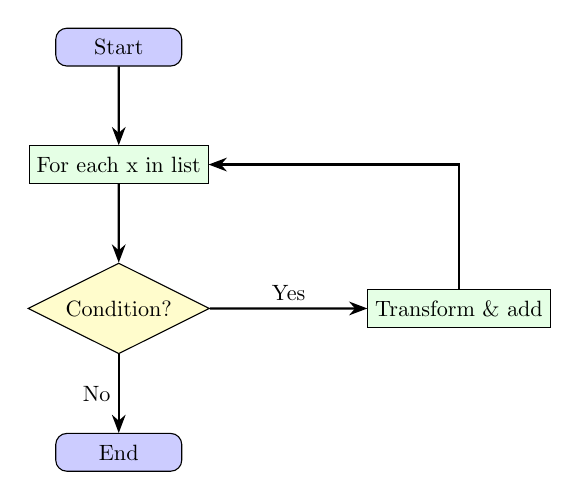
\begin{tikzpicture}[node distance=1cm, scale=0.8, every node/.style={scale=0.8}]
            \node (start) [startstop] {Start};
            \node (loop) [process, below=of start] {For each x in list};
            \node (cond) [decision, below=of loop] {Condition?};
            \node (action) [process, right=2cm of cond] {Transform \& add};
            \node (end) [startstop, below=of cond] {End};
            
            \draw[arrow] (start) -- (loop);
            \draw[arrow] (loop) -- (cond);
            \draw[arrow] (cond) -- node[above] {Yes} (action);
            \draw[arrow] (cond) -- node[left] {No} (end);
            \draw[arrow] (action) |- (loop);
        \end{tikzpicture}
    \end{center}
\end{frame}

\begin{frame}[fragile]{Lesson 8 Code Example}
    \small
    \begin{lstlisting}[style=codeStyle]
pic50_values = [5.2, 6.8, 7.3, 4.9, 8.1]

# List comprehension: filter active compounds
actives = [p for p in pic50_values if p >= 6.0]

# Lambda + map: convert pIC50 to IC50 (nM)
ic50_nm = list(map(lambda p: 10**(9-p), pic50_values))

# Filter: highly potent (pIC50 > 7)
potent = list(filter(lambda p: p > 7, pic50_values))

print(actives, ic50_nm, potent)
    \end{lstlisting}
\end{frame}

% --------------------------------------------
% LESSON 8B: LAMBDA & SCOPE
% --------------------------------------------
\begin{frame}{Lesson 8B: Learning Objectives}
    \small
    \textbf{Learning Objectives:}
    \begin{itemize}
        \item Create anonymous functions with lambda
        \item Understand variable scope (local, global, nonlocal)
        \item Use closures for stateful functions
    \end{itemize}
    \vspace{0.5em}
    \textbf{Description:}\\
    Lambda functions are compact, inline functions for simple operations. Understanding scope ensures correct variable access and prevents bugs in complex programs.
    \vspace{0.5em}
    \textbf{Applications:}
    \begin{itemize}
        \item Sort compounds by activity with custom keys
        \item Create quick property calculators
        \item Build stateful counters for batch processing
    \end{itemize}
\end{frame}

\begin{frame}{Lesson 8B: Lambda Functions \& Variable Scope}
    \small
    \textbf{Lambda:} Anonymous single-expression functions\\[0.3em]
    \texttt{lambda args: expression}\\[0.5em]
    \textbf{Variable Scope:}
    \begin{itemize}
        \item \textbf{Local} -- inside function
        \item \textbf{Enclosing} -- outer function (nested)
        \item \textbf{Global} -- module level
        \item \textbf{Built-in} -- Python built-ins
    \end{itemize}
    \vspace{0.3em}
    Use \texttt{global} keyword to modify global variables\\
    Use \texttt{nonlocal} for enclosing scope
\end{frame}

\begin{frame}[fragile]{Lesson 8B Code Example}
    \small
    \begin{lstlisting}[style=codeStyle]
# Lambda functions for molecular properties
to_pic50 = lambda ic50: -math.log10(ic50 * 1e-9)
is_active = lambda p: p >= 6.0

# Sorting compounds by activity
compounds = [("Aspirin", 5.2), ("Ibuprofen", 6.8), ("Drug_X", 7.5)]
compounds.sort(key=lambda x: x[1], reverse=True)

# Variable scope in processing
processed_count = 0  # global

def process_batch():
    global processed_count
    processed_count += 1

def create_counter():
    count = 0
    def increment():
        nonlocal count
        count += 1
        return count
    return increment
    \end{lstlisting}
\end{frame}

% --------------------------------------------
% LESSON 9: DICTIONARIES
% --------------------------------------------
\begin{frame}{Lesson 9: Learning Objectives}
    \small
    \textbf{Learning Objectives:}
    \begin{itemize}
        \item Create and manipulate key-value dictionaries
        \item Access, update, and iterate over dict items
        \item Use dict comprehensions for transformations
    \end{itemize}
    \vspace{0.5em}
    \textbf{Description:}\\
    Dictionaries store data as key-value pairs, enabling fast lookups by name. They are ideal for structured data like compound databases and lookup tables.
    \vspace{0.5em}
    \textbf{Applications:}
    \begin{itemize}
        \item Build compound databases (name $\to$ properties)
        \item Create codon translation tables
        \item Store molecular descriptor lookups
    \end{itemize}
\end{frame}

\begin{frame}{Lesson 9: Dictionaries}
    \small
    Key-value storage, unordered, mutable.\\[0.5em]
    \textbf{Methods:} \texttt{keys()}, \texttt{values()}, \texttt{items()}, \texttt{get()}, \texttt{update()}, \texttt{pop()}, \texttt{popitem()}, \texttt{clear}\\[0.5em]
    \textbf{Scenarios:} Compound database, codon table, property lookup
\end{frame}

\begin{frame}[fragile]{Lesson 9 Code Example}
    \small
    \begin{lstlisting}[style=codeStyle]
compound_db = {
    "Aspirin": {"SMILES": "CC(=O)OC1=CC=CC=C1C(=O)O", "pIC50": 5.2},
    "Caffeine": {"SMILES": "CN1C=NC2=C1C(=O)N(C(=O)N2C)C", "pIC50": 4.8}
}

# Add new compound
compound_db["Ibuprofen"] = {"SMILES": "CC(C)CC1=CC=C(C=C1)C(C)C(=O)O", "pIC50": 6.1}

# Filter actives (dict comprehension)
actives = {k: v for k, v in compound_db.items() if v["pIC50"] >= 5.0}

print(actives)
    \end{lstlisting}
\end{frame}

% --------------------------------------------
% LESSON 10: FILE HANDLING
% --------------------------------------------
\begin{frame}{Lesson 10: Learning Objectives}
    \small
    \textbf{Learning Objectives:}
    \begin{itemize}
        \item Read and write text files using open()
        \item Use context managers (with) for safe file handling
        \item Parse structured file formats (CSV, FASTA)
    \end{itemize}
    \vspace{0.5em}
    \textbf{Description:}\\
    File I/O enables programs to read input data and save results. Essential for working with compound datasets (CSV, SDF) and biological sequences (FASTA).
    \vspace{0.5em}
    \textbf{Applications:}
    \begin{itemize}
        \item Read/write compound CSV files
        \item Parse FASTA sequence files
        \item Export filtered results for downstream analysis
    \end{itemize}
\end{frame}

\begin{frame}{Lesson 10: File Handling}
    \small
    Read/write text files.\\[0.5em]
    \textbf{Methods:} \texttt{open()}, \texttt{read()}, \texttt{readline()}, \texttt{readlines()}, \texttt{write()}, \texttt{writelines()}, \texttt{close()}\\[0.5em]
    Use \texttt{with} for automatic closing
    \vspace{0.5em}
    \begin{center}
        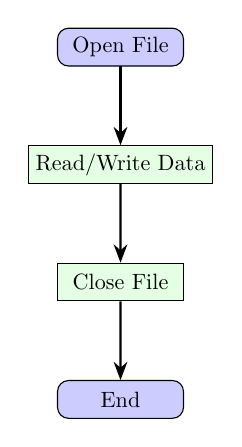
\begin{tikzpicture}[node distance=1cm, scale=0.8, every node/.style={scale=0.8}]
            \node (start) [startstop] {Open File};
            \node (read) [process, below=of start] {Read/Write Data};
            \node (close) [process, below=of read] {Close File};
            \node (end) [startstop, below=of close] {End};
            
            \draw[arrow] (start) -- (read);
            \draw[arrow] (read) -- (close);
            \draw[arrow] (close) -- (end);
        \end{tikzpicture}
    \end{center}
\end{frame}

\begin{frame}[fragile]{Lesson 10 Code Example}
    \small
    \begin{lstlisting}[style=codeStyle]
# Write compound data to CSV
with open("compounds.csv", "w") as f:
    f.write("name,smiles,pIC50\n")
    f.write("Aspirin,CC(=O)OC1=CC=CC=C1C(=O)O,5.2\n")

# Read FASTA file
with open("sequence.fasta", "r") as f:
    header = f.readline().strip()  # >sequence_id
    sequence = ""
    for line in f:
        sequence += line.strip()
    \end{lstlisting}
\end{frame}

% --------------------------------------------
% LESSON 11: NUMPY ARRAYS
% --------------------------------------------
\begin{frame}{Lesson 11: Learning Objectives}
    \small
    \textbf{Learning Objectives:}
    \begin{itemize}
        \item Create and manipulate NumPy arrays
        \item Perform vectorized mathematical operations
        \item Use boolean indexing for data filtering
    \end{itemize}
    \vspace{0.5em}
    \textbf{Description:}\\
    NumPy provides efficient N-dimensional arrays for numerical computing. Vectorized operations are orders of magnitude faster than Python loops for large datasets.
    \vspace{0.5em}
    \textbf{Applications:}
    \begin{itemize}
        \item Store molecular descriptor matrices
        \item Normalize and scale feature data
        \item Compute statistics on activity arrays
    \end{itemize}
\end{frame}

\begin{frame}{Lesson 11: NumPy Arrays}
    \small
    NumPy arrays for efficient numerical computation\\[0.5em]
    \textbf{Key Data Structures:}
    \begin{itemize}
        \item \texttt{ndarray} -- N-dimensional array (homogeneous data)
        \item Supports 1D (vector), 2D (matrix), nD (tensor)
    \end{itemize}
    \vspace{0.3em}
    \textbf{Array Creation:}
    \begin{itemize}
        \item \texttt{np.array()} -- from list/tuple
        \item \texttt{np.zeros()}, \texttt{np.ones()} -- filled arrays
        \item \texttt{np.arange()}, \texttt{np.linspace()} -- sequences
        \item \texttt{np.random.rand()} -- random arrays
    \end{itemize}
\end{frame}

\begin{frame}{Lesson 11: NumPy Properties \& Operations}
    \small
    \textbf{Array Properties:}
    \begin{itemize}
        \item \texttt{shape} -- dimensions (rows, cols)
        \item \texttt{dtype} -- data type (int64, float64)
        \item \texttt{ndim} -- number of dimensions
        \item \texttt{size} -- total elements
    \end{itemize}
    \vspace{0.3em}
    \textbf{Key Operations:}
    \begin{itemize}
        \item Element-wise: \texttt{+}, \texttt{-}, \texttt{*}, \texttt{/}, \texttt{**}
        \item Aggregation: \texttt{sum()}, \texttt{mean()}, \texttt{std()}, \texttt{min()}, \texttt{max()}
        \item Reshaping: \texttt{reshape()}, \texttt{flatten()}, \texttt{transpose()}
        \item Indexing: slicing, boolean masks, fancy indexing
    \end{itemize}
\end{frame}

\begin{frame}[fragile]{Lesson 11 Code Example}
    \small
    \begin{lstlisting}[style=codeStyle]
import numpy as np

# Array creation
arr = np.array([[1, 2, 3], [4, 5, 6], [7, 8, 9]])
zeros = np.zeros((2, 3))      # 2x3 array of zeros
ones = np.ones((3, 3))        # 3x3 array of ones
seq = np.arange(0, 10, 2)     # [0, 2, 4, 6, 8]

# Properties
print(arr.shape, arr.dtype, arr.ndim)

# Operations
print(arr * 2)                # element-wise multiply
print(arr.sum(axis=0))        # sum per column
print(arr.mean(axis=1))       # mean per row

# Boolean indexing
mask = arr > 5
print(arr[mask])              # [6, 7, 8, 9]
    \end{lstlisting}
\end{frame}

% --------------------------------------------
% LESSON 11B: PANDAS DATA STRUCTURES
% --------------------------------------------
\begin{frame}{Lesson 11B: Learning Objectives}
    \small
    \textbf{Learning Objectives:}
    \begin{itemize}
        \item Create Series and DataFrame structures
        \item Filter, group, and aggregate tabular data
        \item Read/write data from CSV, Excel, and SDF files
    \end{itemize}
    \vspace{0.5em}
    \textbf{Description:}\\
    Pandas provides labeled data structures for data analysis. DataFrames are the standard for handling compound datasets with mixed data types and missing values.
    \vspace{0.5em}
    \textbf{Applications:}
    \begin{itemize}
        \item Manage compound libraries with properties
        \item Analyze bioactivity data (groupby, statistics)
        \item Merge descriptor and activity datasets
    \end{itemize}
\end{frame}

\begin{frame}{Lesson 11B: Pandas Data Structures}
    \small
    Pandas provides powerful data structures for data analysis\\[0.5em]
    \textbf{Key Data Structures:}
    \begin{itemize}
        \item \texttt{Series} -- 1D labeled array (like a column)
        \item \texttt{DataFrame} -- 2D labeled table (rows \& columns)
    \end{itemize}
    \vspace{0.3em}
    \textbf{Why Pandas?}
    \begin{itemize}
        \item Handles heterogeneous data (mixed types)
        \item Built-in handling of missing values (NaN)
        \item Powerful indexing and filtering
        \item Easy file I/O (CSV, Excel, JSON, SQL)
    \end{itemize}
\end{frame}

\begin{frame}{Lesson 11B: Series \& DataFrame}
    \small
    \textbf{Series:} 1D array with labels (index)
    \begin{itemize}
        \item Created from list, dict, or scalar
        \item Access by label: \texttt{s['a']} or position: \texttt{s[0]}
    \end{itemize}
    \vspace{0.5em}
    \textbf{DataFrame:} 2D table with row/column labels
    \begin{itemize}
        \item Created from dict, list of dicts, or 2D array
        \item Columns = Series
        \item Access column: \texttt{df['col']} or \texttt{df.col}
        \item Access row: \texttt{df.loc['label']} or \texttt{df.iloc[0]}
    \end{itemize}
\end{frame}

\begin{frame}[fragile]{Lesson 11B Code Example (Creation)}
    \small
    \begin{lstlisting}[style=codeStyle]
import pandas as pd

# Series - activity values with compound IDs
activities = pd.Series([5.2, 6.8, 7.3], index=['CMP001', 'CMP002', 'CMP003'])
print(activities['CMP002'])  # 6.8

# DataFrame from compound data
df = pd.DataFrame({
    'Name': ['Aspirin', 'Ibuprofen', 'Caffeine'],
    'SMILES': ['CC(=O)OC1=CC=CC=C1C(=O)O', 'CC(C)CC1=CC=C(C=C1)C(C)C(=O)O', 'CN1C=NC2=C1C(=O)N(C)C(=O)N2C'],
    'pIC50': [5.2, 6.1, 4.8],
    'MW': [180.16, 206.28, 194.19]
})
print(df)

# DataFrame from list of dicts
data = [{'x': 1, 'y': 2}, {'x': 3, 'y': 4}]
df2 = pd.DataFrame(data)
    \end{lstlisting}
\end{frame}

\begin{frame}[fragile]{Lesson 11B Code Example (Operations)}
    \small
    \begin{lstlisting}[style=codeStyle]
import pandas as pd

df = pd.DataFrame({
    'Name': ['Aspirin', 'Ibuprofen', 'Caffeine', 'Drug_X'],
    'pIC50': [5.2, 6.1, 4.8, 7.5],
    'MW': [180.16, 206.28, 194.19, 320.5]
})

# Basic properties
print(df.shape, df.columns, df.dtypes)

# Selection
print(df['Name'])           # single column
print(df[['Name', 'pIC50']])# multiple columns
print(df.loc[0])            # row by label
print(df.iloc[0:2])         # rows by position

# Filtering
actives = df[df['pIC50'] > 6.0]
drug_like = df[df['MW'] < 500]
    \end{lstlisting}
\end{frame}

\begin{frame}[fragile]{Lesson 11B Code Example (Analysis)}
    \small
    \begin{lstlisting}[style=codeStyle]
# Aggregation
print(df['pIC50'].mean())    # average activity
print(df['pIC50'].max())     # most potent
print(df.describe())         # summary statistics

# GroupBy by activity class
df['Class'] = df['pIC50'].apply(lambda x: 'Active' if x >= 6 else 'Inactive')
grouped = df.groupby('Class')['MW'].mean()

# Adding columns
df['IC50_nM'] = 10**(9 - df['pIC50'])

# Sorting by activity
df_sorted = df.sort_values('pIC50', ascending=False)

# Missing data handling
df['LogP'] = [1.2, None, -0.5, 2.3]
df['LogP'].fillna(df['LogP'].mean(), inplace=True)
    \end{lstlisting}
\end{frame}

\begin{frame}[fragile]{Lesson 11B Code Example (File I/O)}
    \small
    \begin{lstlisting}[style=codeStyle]
import pandas as pd

# Read compound data from CSV
df = pd.read_csv('compounds.csv')

# Write filtered actives
df[df['pIC50'] > 6].to_csv('actives.csv', index=False)

# Read from SDF (via RDKit)
from rdkit import Chem
from rdkit.Chem import PandasTools
df = PandasTools.LoadSDF('molecules.sdf')

# Quick data exploration
print(df.head())       # first 5 compounds
print(df.info())       # column types
print(df.describe())   # statistical summary
    \end{lstlisting}
\end{frame}

% --------------------------------------------
% LESSON 12: JSON & REGEX
% --------------------------------------------
\begin{frame}{Lesson 12: Learning Objectives}
    \small
    \textbf{Learning Objectives:}
    \begin{itemize}
        \item Parse and generate JSON data
        \item Write regex patterns for text matching
        \item Extract and validate patterns in sequences
    \end{itemize}
    \vspace{0.5em}
    \textbf{Description:}\\
    JSON is the standard format for web APIs (PubChem, ChEMBL). Regular expressions enable powerful pattern matching for sequence motifs and data validation.
    \vspace{0.5em}
    \textbf{Applications:}
    \begin{itemize}
        \item Query ChEMBL/PubChem REST APIs
        \item Find restriction sites in DNA sequences
        \item Validate SMILES and sequence formats
    \end{itemize}
\end{frame}

\begin{frame}{Lesson 12: JSON \& Regex}
    \small
    \textbf{JSON:} exchange data between systems (PubChem API, ChEMBL)\\
    \texttt{json.loads()}, \texttt{json.dumps()}\\[0.5em]
    \textbf{Regex:} pattern matching for SMILES, sequences\\
    \texttt{re.search()}, \texttt{re.findall()}, \texttt{re.sub()}
\end{frame}

\begin{frame}[fragile]{Lesson 12 Code Example}
    \small
    \begin{lstlisting}[style=codeStyle]
import json
import re

# JSON - PubChem-like data
data = '{"name": "Aspirin", "CID": 2244, "MW": 180.16}'
compound = json.loads(data)
print(compound["name"])

# Regex - find DNA motifs
seq = "ATGCGATCGATCG"
matches = re.findall(r"GATC", seq)  # restriction site
    \end{lstlisting}
\end{frame}

% ============================================
% SECTION 3: ADDITIONAL TOPICS
% ============================================
\section{Additional Topics}

% --------------------------------------------
% LESSON 13: MODULES & PACKAGES
% --------------------------------------------
\begin{frame}{Lesson 13: Learning Objectives}
    \small
    \textbf{Learning Objectives:}
    \begin{itemize}
        \item Import and use modules and packages
        \item Create custom reusable modules
        \item Organize code with proper structure
    \end{itemize}
    \vspace{0.5em}
    \textbf{Description:}\\
    Modules organize code into reusable files. Packages bundle related modules. This enables building maintainable scientific pipelines and sharing code across projects.
    \vspace{0.5em}
    \textbf{Applications:}
    \begin{itemize}
        \item Use RDKit for cheminformatics
        \item Create molecular utility libraries
        \item Build reusable bioinformatics toolkits
    \end{itemize}
\end{frame}

\begin{frame}{Lesson 13: Modules \& Packages}
    \small
    \textbf{Module:} Single Python file with reusable code\\[0.3em]
    \textbf{Package:} Directory containing multiple modules\\[0.5em]
    \textbf{Import Styles:}
    \begin{itemize}
        \item \texttt{import module}
        \item \texttt{from module import function}
        \item \texttt{from module import *}
        \item \texttt{import module as alias}
    \end{itemize}
    \vspace{0.3em}
    \textbf{Creating Modules:} Any \texttt{.py} file is a module\\
    \textbf{\_\_name\_\_:} Use \texttt{if \_\_name\_\_ == "\_\_main\_\_":}
\end{frame}

\begin{frame}[fragile]{Lesson 13 Code Example}
    \small
    \begin{lstlisting}[style=codeStyle]
# Cheminformatics modules
from rdkit import Chem
from rdkit.Chem import Descriptors
import math

# Create molecule utilities (mol_utils.py)
# def calc_lipinski(smiles):
#     mol = Chem.MolFromSmiles(smiles)
#     return {
#         'MW': Descriptors.MolWt(mol),
#         'LogP': Descriptors.MolLogP(mol),
#         'HBD': Descriptors.NumHDonors(mol),
#         'HBA': Descriptors.NumHAcceptors(mol)
#     }

# Main guard
if __name__ == "__main__":
    print("Running QSAR pipeline...")
    \end{lstlisting}
\end{frame}

% ============================================
% SUMMARY & CLOSING
% ============================================
\section{Summary}

\begin{frame}{Course Summary}
    \small
    \textbf{Section 1: Python Basics (Lessons 1--6B)}
    \begin{itemize}
        \item Variables (molecules, bioactivity), Data Types
        \item Operators (IC50 conversion, MW calculation)
        \item Strings (SMILES, DNA sequences)
        \item Conditionals (drug-likeness, activity classification)
        \item Loops (compound libraries, sequence processing)
        \item Functions (property calculators), Error Handling
    \end{itemize}
    \vspace{0.5em}
    \textbf{Section 2: Collections \& Data (Lessons 7--12)}
    \begin{itemize}
        \item Lists (SMILES), Tuples (compound records), Sets (scaffolds), Dicts (compound DB)
        \item List Comprehensions, Lambda for filtering
        \item File Handling (CSV, FASTA, SDF)
        \item NumPy (descriptor matrices), Pandas (compound DataFrames)
        \item JSON (ChEMBL API), Regex (sequence motifs)
    \end{itemize}
    \vspace{0.5em}
    \textbf{Section 3: Additional Topics (Lesson 13)}
    \begin{itemize}
        \item Modules \& Packages (RDKit, Biopython)
    \end{itemize}
\end{frame}

\begin{frame}{Next Steps}
    \small
    \textbf{Practice Resources:}
    \begin{itemize}
        \item Rosalind.info for bioinformatics problems
        \item ChEMBL/PubChem for real compound data
        \item RDKit tutorials for cheminformatics
    \end{itemize}
    \vspace{0.5em}
    \textbf{Topics to Explore Next:}
    \begin{itemize}
        \item Object-Oriented Programming (Molecule classes)
        \item Machine Learning (scikit-learn, XGBoost)
        \item QSAR/QSPR modeling pipelines
        \item Molecular visualization (Py3Dmol, NGLview)
        \item Deep learning (PyTorch, molecular graphs)
        \item Docking \& virtual screening
    \end{itemize}
    \vspace{1em}
    \centering
    \textbf{\Large Questions?}
\end{frame}

\end{document}
